
\documentclass[
	12pt,				
	openright,			
	oneside,			
	a4paper,	
    article,		
	brazil				
	]{abntex2}


% --------- PACOTES ---------
\usepackage{centernot}
\usepackage{amsmath}
\usepackage{amssymb}
\usepackage{lmodern}
\usepackage[T1]{fontenc}
\usepackage[utf8]{inputenc}
\usepackage{lastpage}
\usepackage{indentfirst}
\usepackage{graphicx}
\usepackage{microtype}
\usepackage{mhchem}
\usepackage{fancyhdr}
\usepackage{authoraftertitle}
\usepackage{hyperref}
\usepackage{pgfplots}
% --------- CAPA ---------
\titulo{Reações reversíveis}
\autor{Giuliano}
\local{Recife, PE}
\data{2023}

% --------- INFOS DO PDF ---------
\makeatletter
\hypersetup{
		pdftitle={\@title}, 
		pdfauthor={\@author},
    	pdfsubject={\imprimirpreambulo},
	    pdfcreator={LaTeX},
		pdfkeywords={abnt}{latex}{abntex}{abntex2}, 
		colorlinks=true,       		
    	linkcolor=blue,          	
    	citecolor=blue,        		
    	filecolor=magenta,
		urlcolor=blue,
}
\makeatother


\setlength{\parindent}{1.3cm}
\setlength{\parskip}{0.2cm}

\makeindex

% \graphicspath{{./imgs}}
\begin{document}

% --------- CABEÇALHO ---------
\pagestyle{fancy}
\fancyhead{}
\fancyhead[RO]{\textbf{\MyTitle}}
\fancyfoot{}
\fancyfoot[RO]{\thepage}
\fancyfoot[LO]{\href{https://artigos.kroks.cloud}{artigos.kroks.cloud}}
\renewcommand{\footrulewidth}{0.4pt}

\frenchspacing
\imprimircapa
\tableofcontents
\newpage

% --------- SEÇÕES ---------

\section[Introdução]{Introdução}
Reações reversíveis são aquelas que deslocam-se --- à mesma velocidade --- para os dois sentidos. Por exemplo, veja a seguinte reação:
$$N_{2g} + 3H_{2(g)}\rightleftharpoons2NH_{3(g)}$$
Pode-se notar que há duas setas: a seta voltada à esquerda ($\leftarrow$) (iníco da reação) corresponde à reação inversa; já a voltada à direita ($\rightarrow$) (fim da reação),
à reação direta.

O que está acontecendo é que a amônia ($NH_3$) está sendo decomposta à mesma velocidade e no mesmo meio da qual a reação está acontecendo, passando uma
impressão de que a reação nunca acaba. Num gráfico isso fica assim:

\begin{center}
    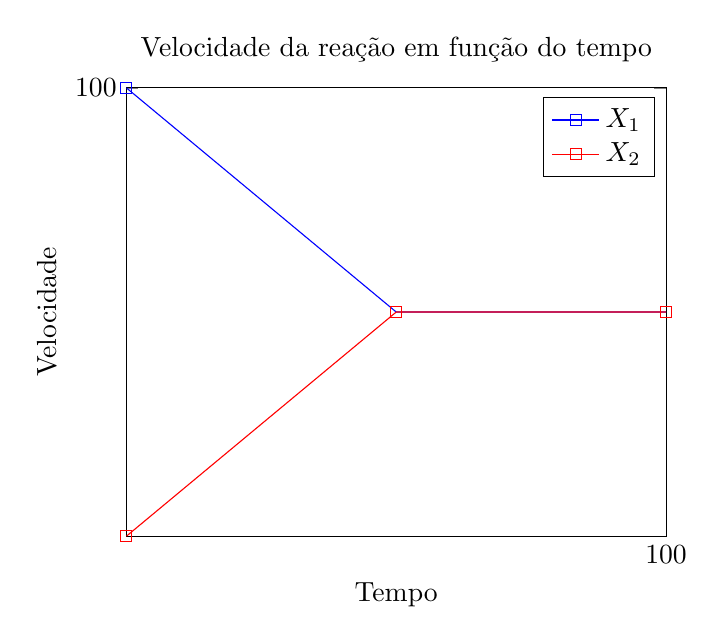
\begin{tikzpicture}
        \begin{axis}[
                title={Velocidade da reação em função do tempo},
                ylabel={Velocidade},
                xlabel={Tempo},
                xmin=0, xmax=100,
                ymin=0, ymax=100,
                xtick={100},
                ytick={100},
            ]
            \addplot[
                color=blue,
                mark=square,
            ]
            coordinates {
                    (0,100)(50,50)(100,50)
                };
            \addplot[
                color=red,
                mark=square,
            ]
            coordinates {
                    (0,0)(50,50)(100,50)
                };
            \legend{$X_1$,$X_2$}
        \end{axis}
    \end{tikzpicture}
\end{center}
O exemplo de cima põe à vista que $X_1$ foi sendo consumido até que, em certo período de tempo, a reação ``tornou-se'' reversível.

\section{Constante de equilíbrio}
 {\tiny*Para este tópico, leve a reação $aA + bB \rightleftharpoons cC + dD$ em conta} \\
A constante do equilíbrio é dada por meio da lei de ação das massas:
$$
    K_c = \frac{[C]^c\cdot[D]^d}{[A]^a\cdot[B]^b}
$$

Por exemplo, com a reação: $N_{2g} + 3H_{2(g)}\rightleftharpoons2NH_{3(g)}$

$$
    K_c = \frac{[NH_3]^2}{[N_2]^1\cdot[H_2^3]}
$$

Os colchetes significam concentração das matérias químicas.
\end{document}